\documentclass[journal,12pt,twocolumn]{IEEEtran}
\usepackage{amsthm}
\usepackage{graphics}
\usepackage{mathrsfs}
\usepackage{txfonts}
\usepackage{stfloats}
\usepackage{pgfplots}
\usepackage{cite}
\usepackage{cases}
\usepackage{mathtools}
\usepackage{caption}
\usepackage{enumerate}
\usepackage{enumitem}
\usepackage{amsmath}
\usepackage[utf8]{inputenc}
\usepackage[english]{babel}
\usepackage{multicol}
\usepackage{multirow}
\usepackage{longtable}
\usepackage{mathtools}
\usepackage{gensymb}
\usepackage{amssymb}
\usepackage{pgfplots}
\usepackage{hyperref}
\usepackage{listings}
\usepackage{color}
\usepackage{array}
\usepackage{calc}
\usepackage{ifthen}
\usepackage{hhline}
\lstset{
%language=C,
frame=single,
breaklines=true,
columns=fullflexible
}

\title{Probability\&RV \\ Assignment-01}
\author{U Anuradha-ee21resch01008}
\date{\today}

\begin{document}

\maketitle
\newpage
\bigskip
\renewcommand{\thefigure}{\theenumi}
\renewcommand{\thetable}{\theenumi}
\textbf{download python code from}
\begin{lstlisting}
 https://github.com/Anuradha-Uggi/Assignments-AI5002-Probability-and-Random-Variables/blob/main/Prob_ass01/rvsp.py
\end{lstlisting}
\textbf{download latex code from}
\begin{lstlisting}
https://github.com/Anuradha-Uggi/Assignments-AI5002-Probability-and-Random-Variables/tree/main/Prob_ass01/ProbSp.tex
\end{lstlisting}


\section{Problem(9.3)}
random variable $z=n_1-n_2$, where $n_1,n_2\sim N(0,1)$
prove that z is a Gaussian random variable and find mean and variance of z.comment it.
\section{Solution}
Moment Generating Function (MGF)is given by 
\begin{equation}
   M_t(s)=E[e^{-st}] 
\end{equation}\\
pdf of $n_1$ is 
\begin{equation}
    f_{N_1}(n_1)=\frac{1}{\sqrt{2\pi}\sigma_{n_1}}e^{-\frac{(n_1-\mu_{n_1})^2}{2\sigma_{n_1}^2}}
\end{equation} \\
MGF of $n_1$ is \\
$M_{n_1}(s)=\int_{-\infty}^{\infty}e^{-s n_1}f({n_1}) d{n_1} $ \\
above equation represents Laplace Transform of f(n1),we know that the L.T of $f_{N_1}(n_1)$ is
\begin{equation}
      M_{n_1}(s)=e^{-s\mu_{n_1}}e^{-\frac{s^2\sigma_{n_1}^2}{2}}
\end{equation}
similarly pdf of $n_2$ is
\begin{equation}
    f_{N_2}(n_2)=\frac{1}{\sqrt{2\pi}\sigma_{n_2}}e^{-\frac{(n_2-\mu_{n_2})^2}{2\sigma_{n_2}^2}}
\end{equation}
MGF of $f_{N_2}(n_2)$
\begin{equation}
    M_{n_2}(s)=e^{-s\mu_{n_2}}e^{-\frac{s^2\sigma_{n_2}^2}{2}}
\end{equation}
MGF of z can be written as \\
$M_z(s)=E[e^{-(n_1+n_2)s}]=M_{n_1}(s)\times M_{n_2}(s)$\\
by substituting eq(3) and eq(5) in $M_z(s)$\\
\begin{equation}
    M_z(s)=e^{-s(\mu_{n_1}+\mu_{n_2})}e^{-\frac{s^2(\sigma_{n_1}^2+\sigma_{n_2}^2)}{2}}
\end{equation} 
\begin{equation}
   \therefore f_Z(z)=\frac{1}{\sqrt{2\pi}\sigma_z}e^{-\frac{(z-(\mu_{n_1}+\mu_{n_2}))^2}{2(\sigma_{n_1}^2+\sigma_{n_2}^2)}}
\end{equation}
lets substitute values $\mu_{n_1}=\mu_{n_2}=0$ and $\sigma_{n_1}^2=\sigma_{n_2}^2=1$ in above equations
\begin{equation}
    f_{N_1}(n_1)=\frac{1}{\sqrt{2\pi}}e^{-\frac{n_1^2}{2}}
\end{equation}
\begin{equation}
    f_{N_2}(n_2)=\frac{1}{\sqrt{2\pi}}e^{-\frac{n_2^2}{2}}
\end{equation}
\begin{equation}
    M_{n_1}(s)=e^{-\frac{s^2}{2}}
\end{equation}
\begin{equation}
    M_{n_2}(s)=e^{-\frac{s^2}{2}}
\end{equation}
\begin{equation}
    M_z(s)=e^{-s^2}
\end{equation}\\
finally
\begin{equation}
  f_Z(z)=\frac{1}{\sqrt{2\pi}}e^{-\frac{z^2}{4}}
\end{equation}
\begin{tikzpicture}
   \begin{axis}[axis lines=left,xlabel={R.V},ylabel={PDFs}]
     \addplot[domain=-5:5, samples=20,color=red]{e^(-(x^2)/2)};
     \addlegendentry{$e^{-\frac{n_1^2}{2}}$}
     \addplot[domain=-5:5, samples=20,color=green]{e^(-(x^2)/2};
      \addlegendentry{$e^{-\frac{n_2^2}{2}}$}
   \addplot[domain=-10:10, samples=40,color=blue]{e^(-(x^2)/4)/2};
   \addlegendentry{$\frac{e^{-\frac{z^2}{4}}}{2}$}
 \end{axis}
\end{tikzpicture} \\

\begin{figure}
    \centering
    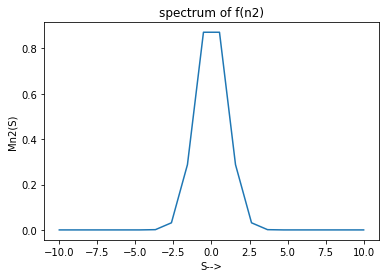
\includegraphics[width=0.5 \textwidth]{rvsp1.png}
\end{figure}
\section{Conclusion}
Random variable which is either sum or difference of two standard normal variables is also a normal variable.\\
$ \mu_z=\mu_{n_1}+\mu_{n_2}=0$ and $\sigma_z^2=\sigma_{n_1}^2+\sigma_{n_2}^2=2$


\end{document}
